% Options for packages loaded elsewhere
\PassOptionsToPackage{unicode}{hyperref}
\PassOptionsToPackage{hyphens}{url}
\PassOptionsToPackage{dvipsnames,svgnames,x11names}{xcolor}
%
\documentclass[
  letterpaper,
  DIV=11,
  numbers=noendperiod]{scrartcl}

\usepackage{amsmath,amssymb}
\usepackage{iftex}
\ifPDFTeX
  \usepackage[T1]{fontenc}
  \usepackage[utf8]{inputenc}
  \usepackage{textcomp} % provide euro and other symbols
\else % if luatex or xetex
  \usepackage{unicode-math}
  \defaultfontfeatures{Scale=MatchLowercase}
  \defaultfontfeatures[\rmfamily]{Ligatures=TeX,Scale=1}
\fi
\usepackage{lmodern}
\ifPDFTeX\else  
    % xetex/luatex font selection
\fi
% Use upquote if available, for straight quotes in verbatim environments
\IfFileExists{upquote.sty}{\usepackage{upquote}}{}
\IfFileExists{microtype.sty}{% use microtype if available
  \usepackage[]{microtype}
  \UseMicrotypeSet[protrusion]{basicmath} % disable protrusion for tt fonts
}{}
\makeatletter
\@ifundefined{KOMAClassName}{% if non-KOMA class
  \IfFileExists{parskip.sty}{%
    \usepackage{parskip}
  }{% else
    \setlength{\parindent}{0pt}
    \setlength{\parskip}{6pt plus 2pt minus 1pt}}
}{% if KOMA class
  \KOMAoptions{parskip=half}}
\makeatother
\usepackage{xcolor}
\setlength{\emergencystretch}{3em} % prevent overfull lines
\setcounter{secnumdepth}{-\maxdimen} % remove section numbering
% Make \paragraph and \subparagraph free-standing
\makeatletter
\ifx\paragraph\undefined\else
  \let\oldparagraph\paragraph
  \renewcommand{\paragraph}{
    \@ifstar
      \xxxParagraphStar
      \xxxParagraphNoStar
  }
  \newcommand{\xxxParagraphStar}[1]{\oldparagraph*{#1}\mbox{}}
  \newcommand{\xxxParagraphNoStar}[1]{\oldparagraph{#1}\mbox{}}
\fi
\ifx\subparagraph\undefined\else
  \let\oldsubparagraph\subparagraph
  \renewcommand{\subparagraph}{
    \@ifstar
      \xxxSubParagraphStar
      \xxxSubParagraphNoStar
  }
  \newcommand{\xxxSubParagraphStar}[1]{\oldsubparagraph*{#1}\mbox{}}
  \newcommand{\xxxSubParagraphNoStar}[1]{\oldsubparagraph{#1}\mbox{}}
\fi
\makeatother


\providecommand{\tightlist}{%
  \setlength{\itemsep}{0pt}\setlength{\parskip}{0pt}}\usepackage{longtable,booktabs,array}
\usepackage{calc} % for calculating minipage widths
% Correct order of tables after \paragraph or \subparagraph
\usepackage{etoolbox}
\makeatletter
\patchcmd\longtable{\par}{\if@noskipsec\mbox{}\fi\par}{}{}
\makeatother
% Allow footnotes in longtable head/foot
\IfFileExists{footnotehyper.sty}{\usepackage{footnotehyper}}{\usepackage{footnote}}
\makesavenoteenv{longtable}
\usepackage{graphicx}
\makeatletter
\newsavebox\pandoc@box
\newcommand*\pandocbounded[1]{% scales image to fit in text height/width
  \sbox\pandoc@box{#1}%
  \Gscale@div\@tempa{\textheight}{\dimexpr\ht\pandoc@box+\dp\pandoc@box\relax}%
  \Gscale@div\@tempb{\linewidth}{\wd\pandoc@box}%
  \ifdim\@tempb\p@<\@tempa\p@\let\@tempa\@tempb\fi% select the smaller of both
  \ifdim\@tempa\p@<\p@\scalebox{\@tempa}{\usebox\pandoc@box}%
  \else\usebox{\pandoc@box}%
  \fi%
}
% Set default figure placement to htbp
\def\fps@figure{htbp}
\makeatother

\KOMAoption{captions}{tableheading}
\makeatletter
\@ifpackageloaded{caption}{}{\usepackage{caption}}
\AtBeginDocument{%
\ifdefined\contentsname
  \renewcommand*\contentsname{Содержание}
\else
  \newcommand\contentsname{Содержание}
\fi
\ifdefined\listfigurename
  \renewcommand*\listfigurename{Список иллюстраций}
\else
  \newcommand\listfigurename{Список иллюстраций}
\fi
\ifdefined\listtablename
  \renewcommand*\listtablename{Список таблиц}
\else
  \newcommand\listtablename{Список таблиц}
\fi
\ifdefined\figurename
  \renewcommand*\figurename{Рисунок}
\else
  \newcommand\figurename{Рисунок}
\fi
\ifdefined\tablename
  \renewcommand*\tablename{Таблица}
\else
  \newcommand\tablename{Таблица}
\fi
}
\@ifpackageloaded{float}{}{\usepackage{float}}
\floatstyle{ruled}
\@ifundefined{c@chapter}{\newfloat{codelisting}{h}{lop}}{\newfloat{codelisting}{h}{lop}[chapter]}
\floatname{codelisting}{Список}
\newcommand*\listoflistings{\listof{codelisting}{Листинги}}
\makeatother
\makeatletter
\makeatother
\makeatletter
\@ifpackageloaded{caption}{}{\usepackage{caption}}
\@ifpackageloaded{subcaption}{}{\usepackage{subcaption}}
\makeatother

\ifLuaTeX
\usepackage[bidi=basic]{babel}
\else
\usepackage[bidi=default]{babel}
\fi
\babelprovide[main,import]{russian}
% get rid of language-specific shorthands (see #6817):
\let\LanguageShortHands\languageshorthands
\def\languageshorthands#1{}
\usepackage{bookmark}

\IfFileExists{xurl.sty}{\usepackage{xurl}}{} % add URL line breaks if available
\urlstyle{same} % disable monospaced font for URLs
\hypersetup{
  pdflang={ru-RU},
  colorlinks=true,
  linkcolor={blue},
  filecolor={Maroon},
  citecolor={Blue},
  urlcolor={Blue},
  pdfcreator={LaTeX via pandoc}}


\author{}
\date{}

\begin{document}


\begin{center}\rule{0.5\linewidth}{0.5pt}\end{center}

execute: eval: false echo: true

\subsection{Author}\label{author}

author: name: Тарасова Алина Андреевна degrees: студент email:
1132236013@rudn.ru affiliation: - name: Российский университет дружбы
народов country: Российская Федерация postal-code: 117198 city: Москва
address: ул. Миклухо-Маклая, д. 6

\subsection{Title}\label{title}

title: Лабораторная работа №2 subtitle: Модели SIR и Лотки-Вольтерры
license: CC BY date: today date-format: ``YYYY-MM-DD'' ---

\section{Информация}\label{ux438ux43dux444ux43eux440ux43cux430ux446ux438ux44f}

\subsection{Докладчик}\label{ux434ux43eux43aux43bux430ux434ux447ux438ux43a}

\begin{itemize}
\tightlist
\item
  Тарасова Алина Андреевна
\item
  студент 2 курса кафедры ММИИИ
\item
  Российский университет дружбы народов им. П. Лумумбы
\item
  \href{mailto:1132236013@rudn.ru}{\nolinkurl{1132236013@rudn.ru}}
\item
  \url{https://gitverse.ru/aatarasova}
\item
  \url{https://github.com/aatarasova}
\end{itemize}

\section{Вводная
часть}\label{ux432ux432ux43eux434ux43dux430ux44f-ux447ux430ux441ux442ux44c}

\subsection{Актуальность}\label{ux430ux43aux442ux443ux430ux43bux44cux43dux43eux441ux442ux44c}

\begin{itemize}
\tightlist
\item
  Математическое моделирование --- ключевой инструмент анализа сложных
  систем
\item
  Модель SIR позволяет прогнозировать развитие эпидемий
\item
  Модель Лотки-Вольтерры описывает динамику популяций в экологии
\item
  Julia --- современный язык для научных вычислений
\end{itemize}

\subsection{Объект и предмет
исследования}\label{ux43eux431ux44aux435ux43aux442-ux438-ux43fux440ux435ux434ux43cux435ux442-ux438ux441ux441ux43bux435ux434ux43eux432ux430ux43dux438ux44f}

\begin{itemize}
\tightlist
\item
  Объект: Процессы распространения инфекций и взаимодействия популяций
\item
  Предмет:

  \begin{itemize}
  \tightlist
  \item
    Модель SIR (эпидемиология)
  \item
    Модель Лотки-Вольтерры (экология)
  \item
    Численные методы решения ОДУ в Julia
  \end{itemize}
\end{itemize}

\subsection{Цели и
задачи}\label{ux446ux435ux43bux438-ux438-ux437ux430ux434ux430ux447ux438}

\begin{itemize}
\tightlist
\item
  Изучить фундаментальные математические модели
\item
  Реализовать численное решение моделей на Julia
\item
  Провести анализ поведения систем при различных параметрах
\item
  Освоить литературное программирование с Literate.jl
\end{itemize}

\subsection{Материалы и
методы}\label{ux43cux430ux442ux435ux440ux438ux430ux43bux44b-ux438-ux43cux435ux442ux43eux434ux44b}

\begin{itemize}
\tightlist
\item
  Язык программирования Julia
\item
  Пакеты: \texttt{DifferentialEquations.jl}, \texttt{Plots.jl},
  \texttt{DrWatson.jl}
\item
  Литературное программирование: \texttt{Literate.jl}
\item
  Оформление отчётов: \texttt{Quarto}
\end{itemize}

\section{Теоретическая
часть}\label{ux442ux435ux43eux440ux435ux442ux438ux447ux435ux441ux43aux430ux44f-ux447ux430ux441ux442ux44c}

\subsection{Модель SIR}\label{ux43cux43eux434ux435ux43bux44c-sir}

\textbf{Три группы людей:} - \textbf{S} (Susceptible) --- восприимчивые
- \textbf{I} (Infectious) --- инфицированные - \textbf{R} (Recovered)
--- выздоровевшие

\textbf{Система уравнений:} \[ \frac{dS}{dt} = -\frac{\beta I S}{N} \]
\[ \frac{dI}{dt} = \frac{\beta I S}{N} - \gamma I \]
\[ \frac{dR}{dt} = \gamma I \]

\subsection{Параметры модели
SIR}\label{ux43fux430ux440ux430ux43cux435ux442ux440ux44b-ux43cux43eux434ux435ux43bux438-sir}

\begin{longtable}[]{@{}ll@{}}
\toprule\noalign{}
Параметр & Описание \\
\midrule\noalign{}
\endhead
\bottomrule\noalign{}
\endlastfoot
\(\beta\) & Коэффициент заражения \\
\(\gamma\) & Коэффициент выздоровления \\
\(R_0 = \beta/\gamma\) & Базовое репродуктивное число \\
\end{longtable}

\textbf{Критерии:} - \(R_0 > 1\) --- эпидемия растёт - \(R_0 < 1\) ---
эпидемия затухает

\subsection{Модель
Лотки-Вольтерры}\label{ux43cux43eux434ux435ux43bux44c-ux43bux43eux442ux43aux438-ux432ux43eux43bux44cux442ux435ux440ux440ux44b}

\textbf{Две популяции:} - \(x\) --- жертвы (например, зайцы) - \(y\) ---
хищники (например, волки)

\textbf{Система уравнений:} \[ \frac{dx}{dt} = \alpha x - \beta x y \]
\[ \frac{dy}{dt} = \delta x y - \gamma y \]

\subsection{Параметры модели
Лотки-Вольтерры}\label{ux43fux430ux440ux430ux43cux435ux442ux440ux44b-ux43cux43eux434ux435ux43bux438-ux43bux43eux442ux43aux438-ux432ux43eux43bux44cux442ux435ux440ux440ux44b}

\begin{longtable}[]{@{}ll@{}}
\toprule\noalign{}
Параметр & Описание \\
\midrule\noalign{}
\endhead
\bottomrule\noalign{}
\endlastfoot
\(\alpha\) & Рождаемость жертв \\
\(\beta\) & Поедание жертв хищниками \\
\(\delta\) & Конверсия пищи в хищников \\
\(\gamma\) & Смертность хищников \\
\end{longtable}

\section{Выполнение лабораторной
работы}\label{ux432ux44bux43fux43eux43bux43dux435ux43dux438ux435-ux43bux430ux431ux43eux440ux430ux442ux43eux440ux43dux43eux439-ux440ux430ux431ux43eux442ux44b}

\subsection{Создание
релиза}\label{ux441ux43eux437ux434ux430ux43dux438ux435-ux440ux435ux43bux438ux437ux430}

\begin{itemize}
\tightlist
\item
  Создан новый релиз v.2.0.0
\end{itemize}

\subsection{Настройка окружения
Julia}\label{ux43dux430ux441ux442ux440ux43eux439ux43aux430-ux43eux43aux440ux443ux436ux435ux43dux438ux44f-julia}

\begin{itemize}
\tightlist
\item
  Запуск Julia и установка пакетов
\end{itemize}

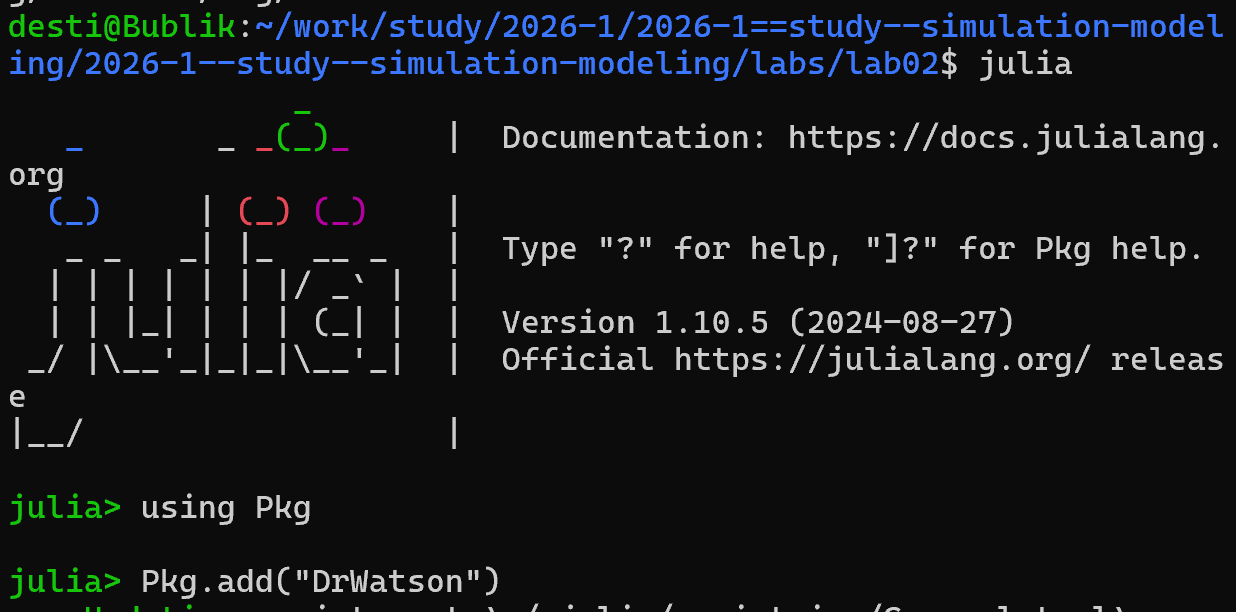
\includegraphics[width=0.7\linewidth,height=\textheight,keepaspectratio]{image/4.png}
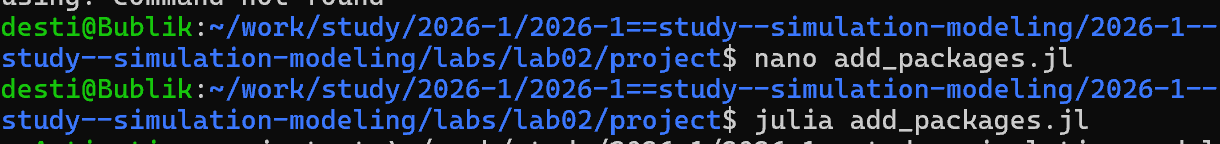
\includegraphics[width=0.7\linewidth,height=\textheight,keepaspectratio]{image/9.png}

\subsection{Создание проекта
DrWatson}\label{ux441ux43eux437ux434ux430ux43dux438ux435-ux43fux440ux43eux435ux43aux442ux430-drwatson}

\begin{itemize}
\tightlist
\item
  Инициализация проекта с DrWatson.jl
\end{itemize}

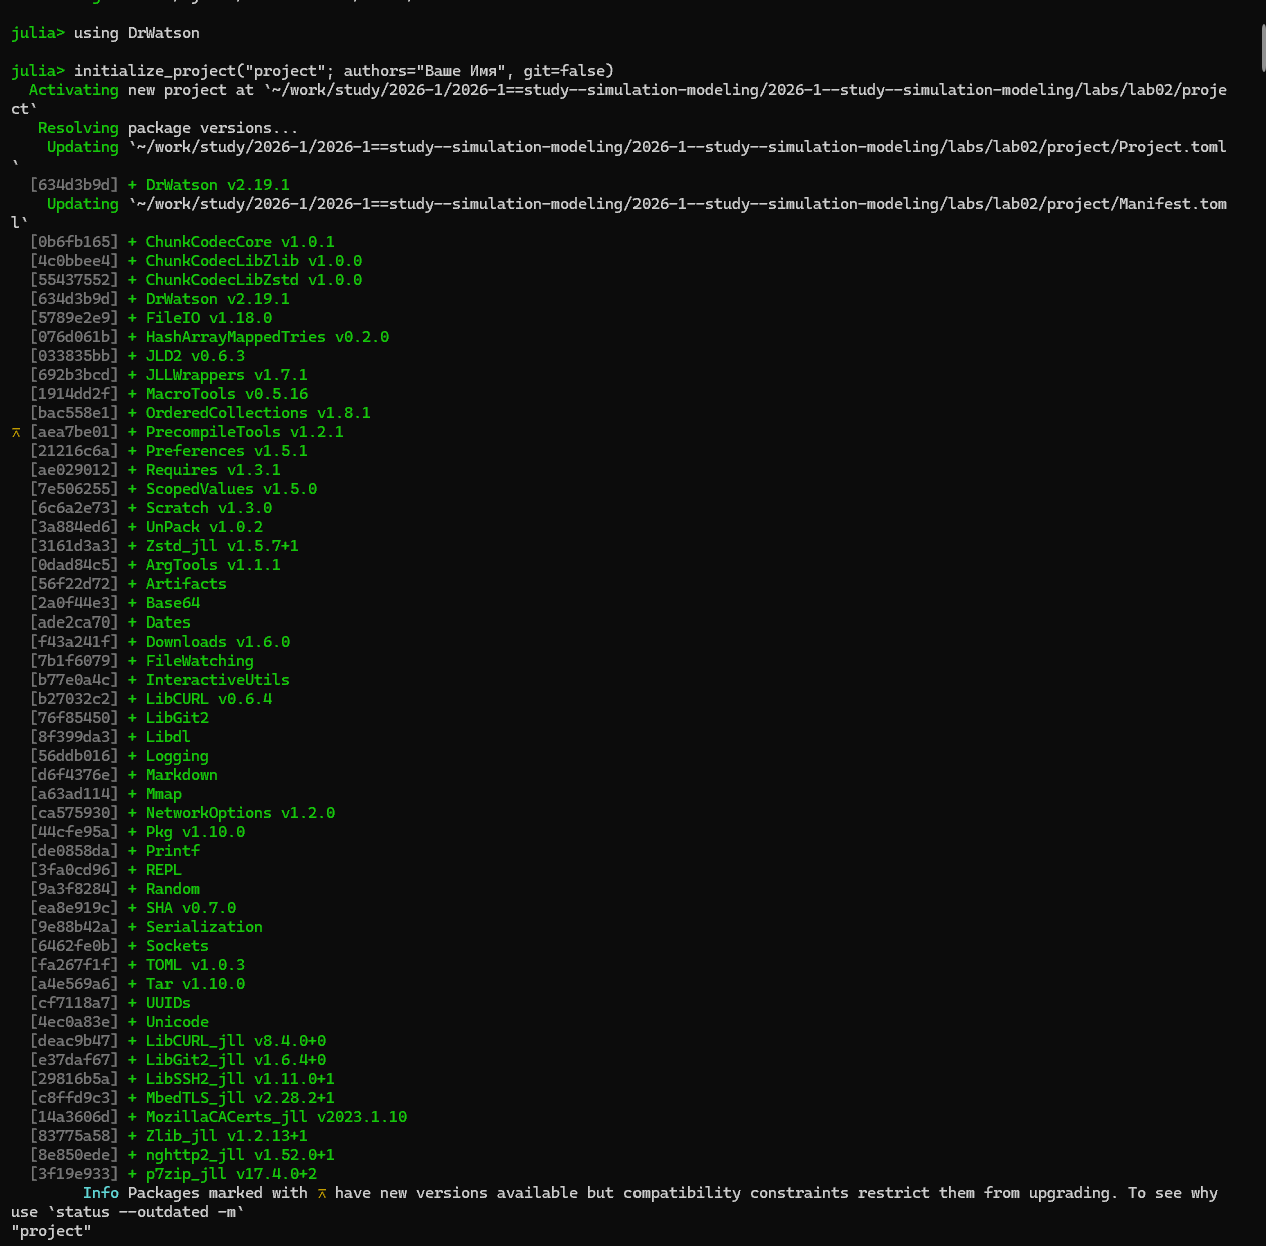
\includegraphics[width=0.7\linewidth,height=\textheight,keepaspectratio]{image/5.png}
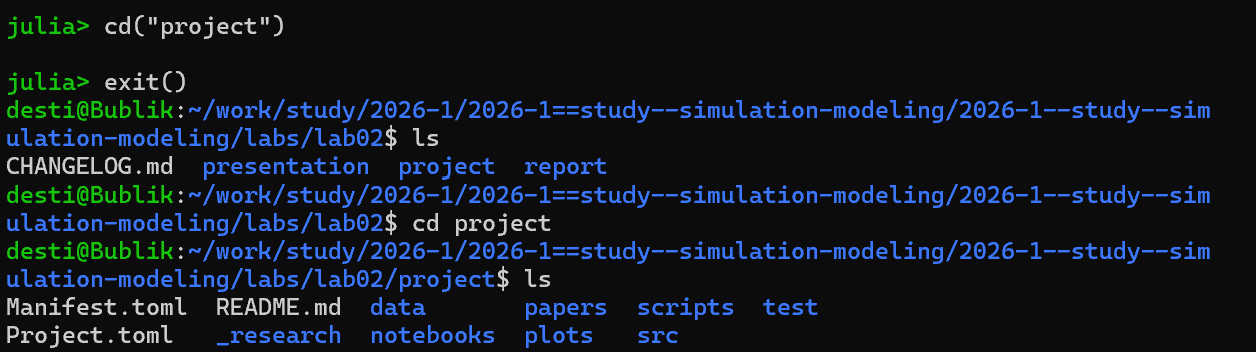
\includegraphics[width=0.7\linewidth,height=\textheight,keepaspectratio]{image/6.png}
ERROR: compilation failed- error Unable to load picture or PDF file
`image/2.png'. \} l.343
\ldots{}\textheight,keepaspectratio{]}\{image/2.png\}

\subsection{Модель SIR}\label{ux43cux43eux434ux435ux43bux44c-sir-1}

\begin{itemize}
\tightlist
\item
  Создание скрипта для модели SIR
\end{itemize}

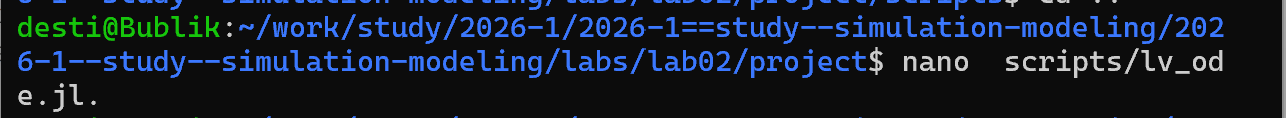
\includegraphics[width=0.7\linewidth,height=\textheight,keepaspectratio]{image/7.png}
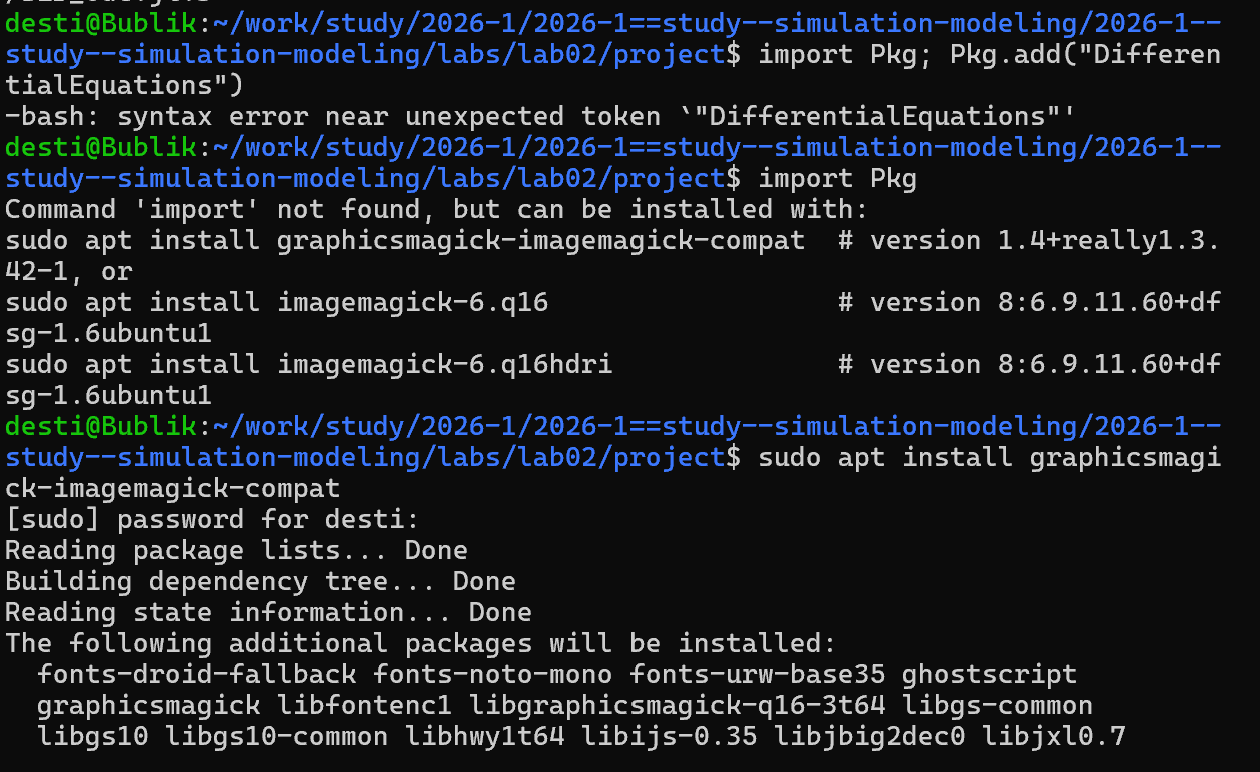
\includegraphics[width=0.7\linewidth,height=\textheight,keepaspectratio]{image/8.png}
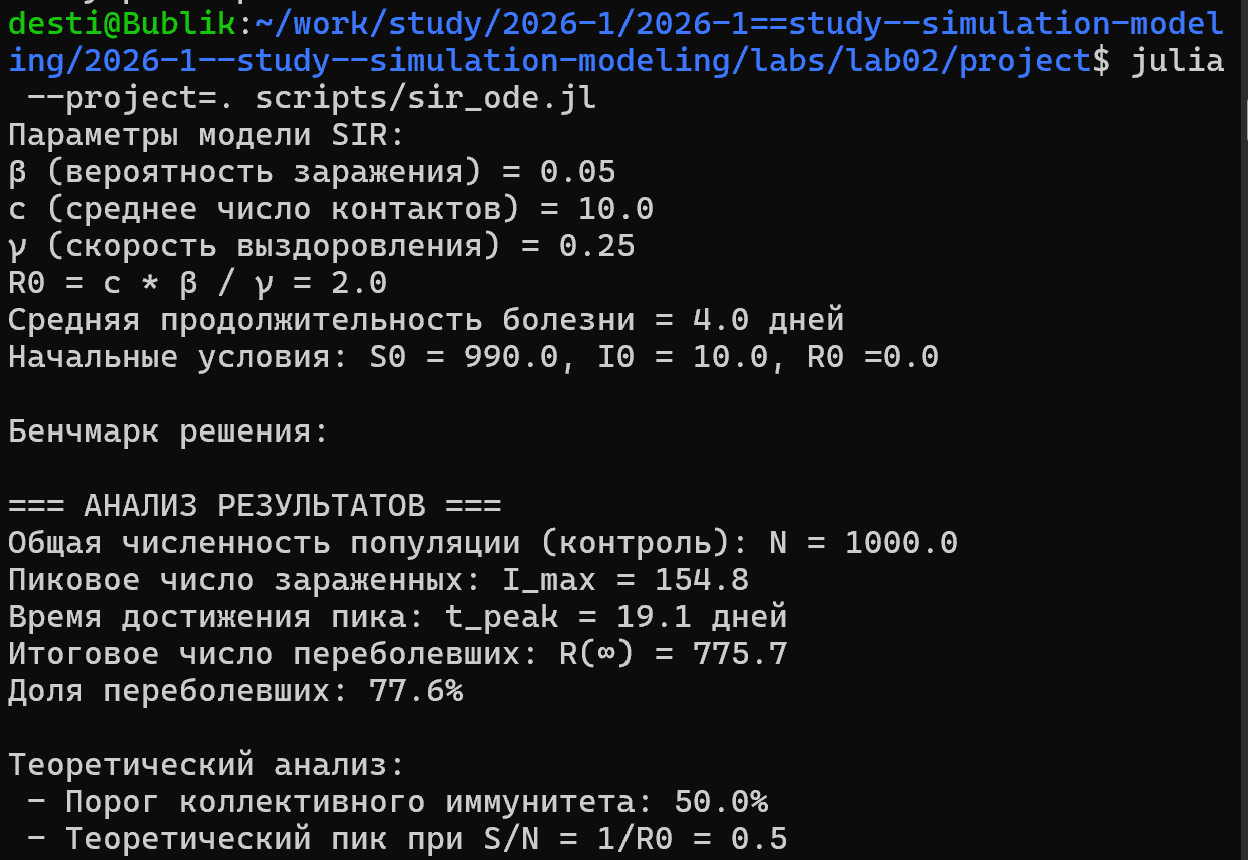
\includegraphics[width=0.7\linewidth,height=\textheight,keepaspectratio]{image/11.png}

\subsection{Модель
Лотки-Вольтерры}\label{ux43cux43eux434ux435ux43bux44c-ux43bux43eux442ux43aux438-ux432ux43eux43bux44cux442ux435ux440ux440ux44b-1}

\begin{itemize}
\tightlist
\item
  Создание скрипта для модели Лотки-Вольтерры
\end{itemize}

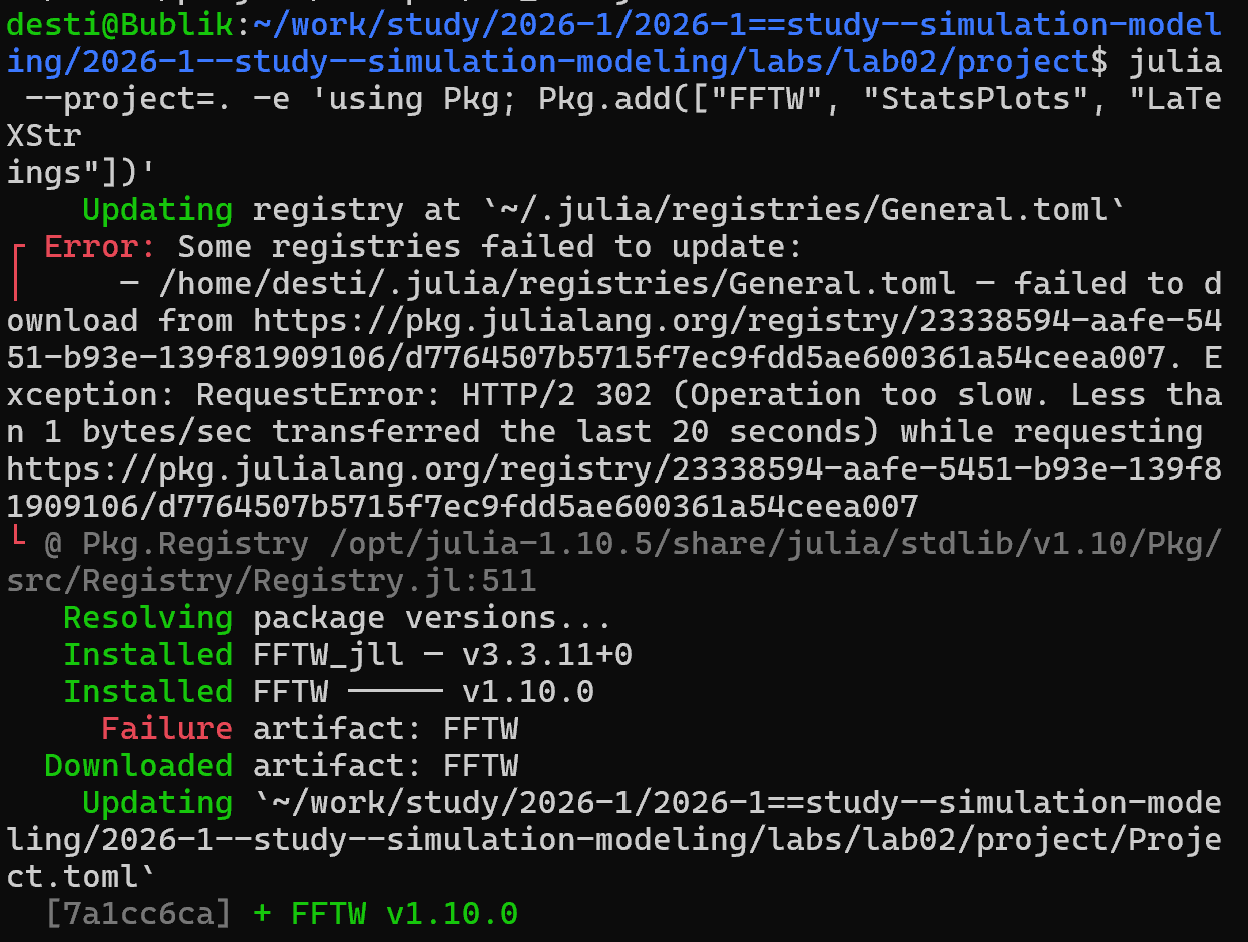
\includegraphics[width=0.7\linewidth,height=\textheight,keepaspectratio]{image/13.png}
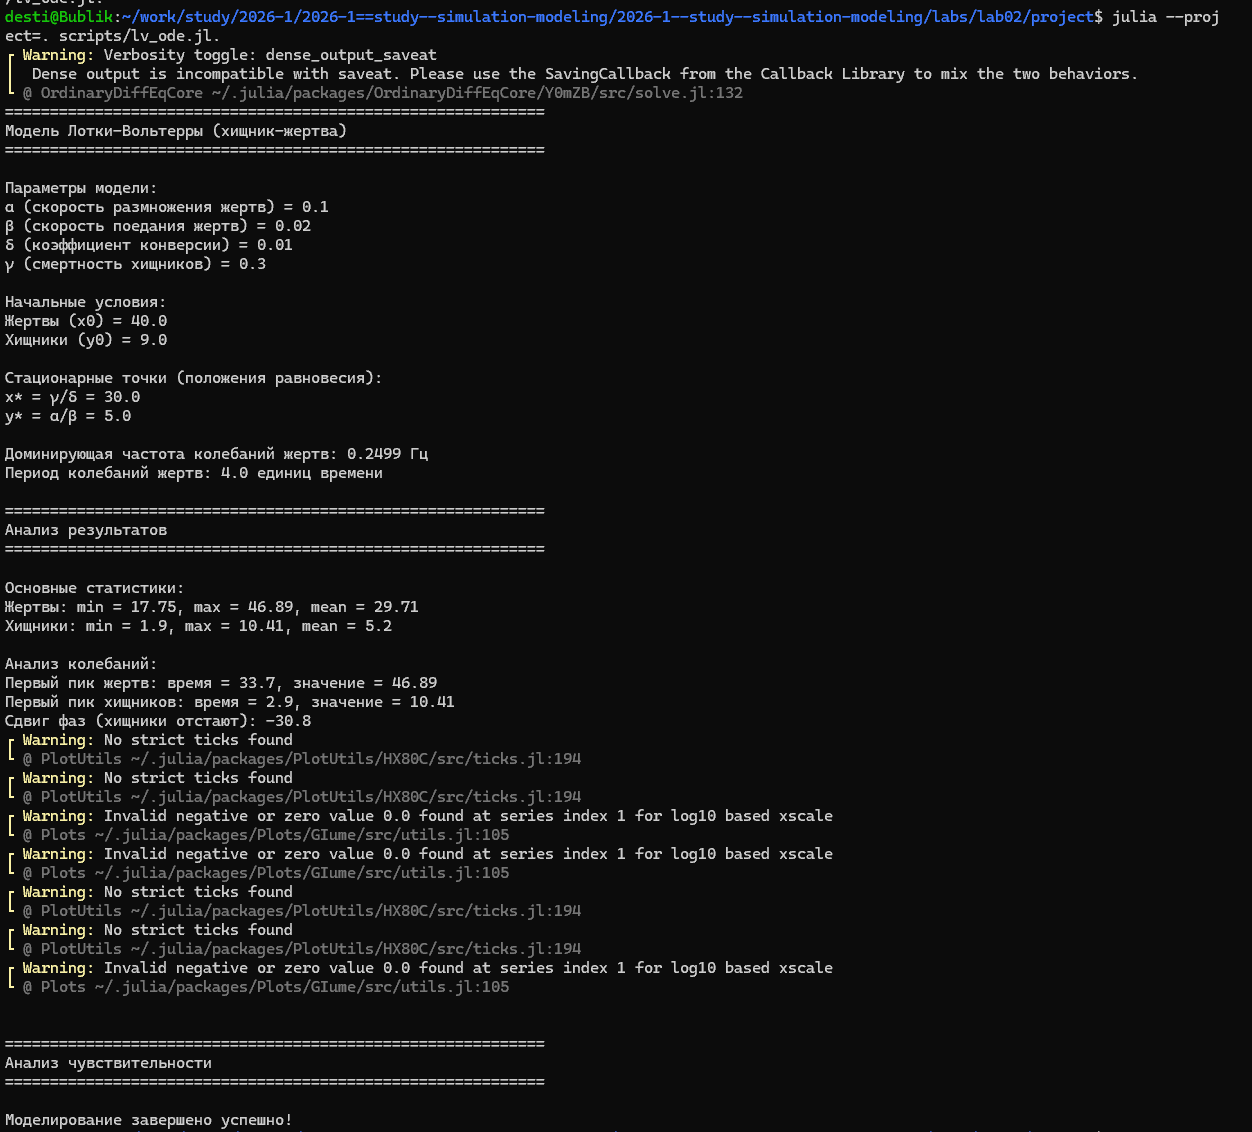
\includegraphics[width=0.7\linewidth,height=\textheight,keepaspectratio]{image/14.png}

\subsection{Создание
отчетов}\label{ux441ux43eux437ux434ux430ux43dux438ux435-ux43eux442ux447ux435ux442ux43eux432}

\begin{itemize}
\tightlist
\item
  Отчет по первой работе
\end{itemize}

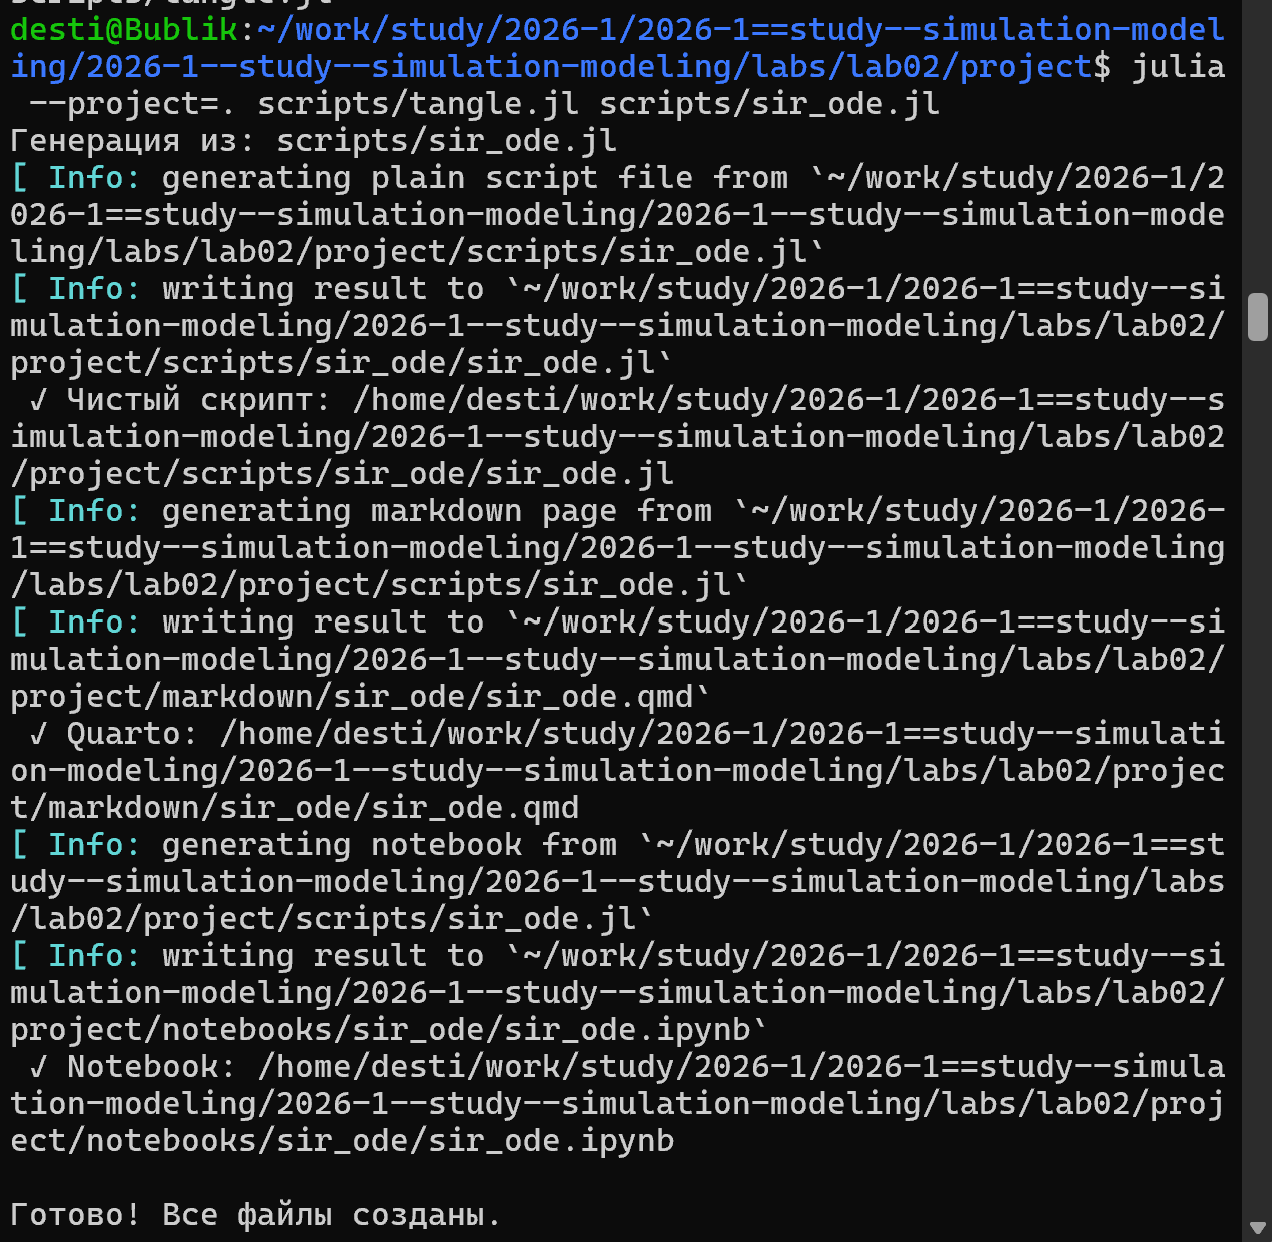
\includegraphics[width=0.7\linewidth,height=\textheight,keepaspectratio]{image/12.png}

\begin{itemize}
\tightlist
\item
  Отчет по второй работе
\end{itemize}

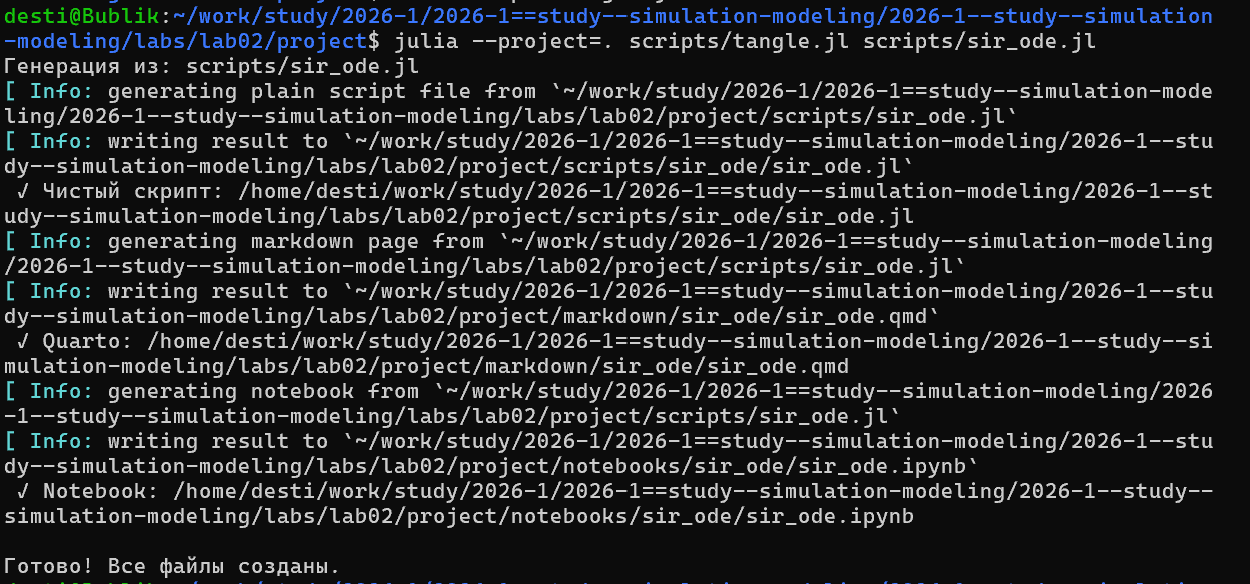
\includegraphics[width=0.7\linewidth,height=\textheight,keepaspectratio]{image/15.png}

\subsection{Работа с Jupyter
notebooks}\label{ux440ux430ux431ux43eux442ux430-ux441-jupyter-notebooks}

\begin{itemize}
\tightlist
\item
  Запуск Jupyter и выполнение notebooks
\end{itemize}

ERROR: compilation failed- error Unable to load picture or PDF file
`image/2.png'. \} l.343
\ldots{}\textheight,keepaspectratio{]}\{image/2.png\}

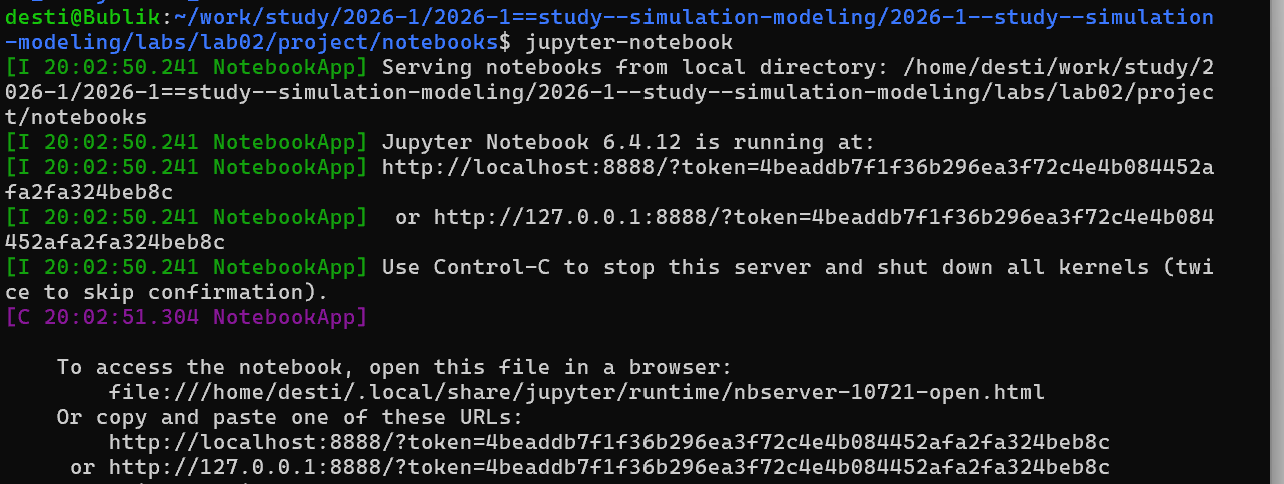
\includegraphics[width=0.7\linewidth,height=\textheight,keepaspectratio]{image/16.png}
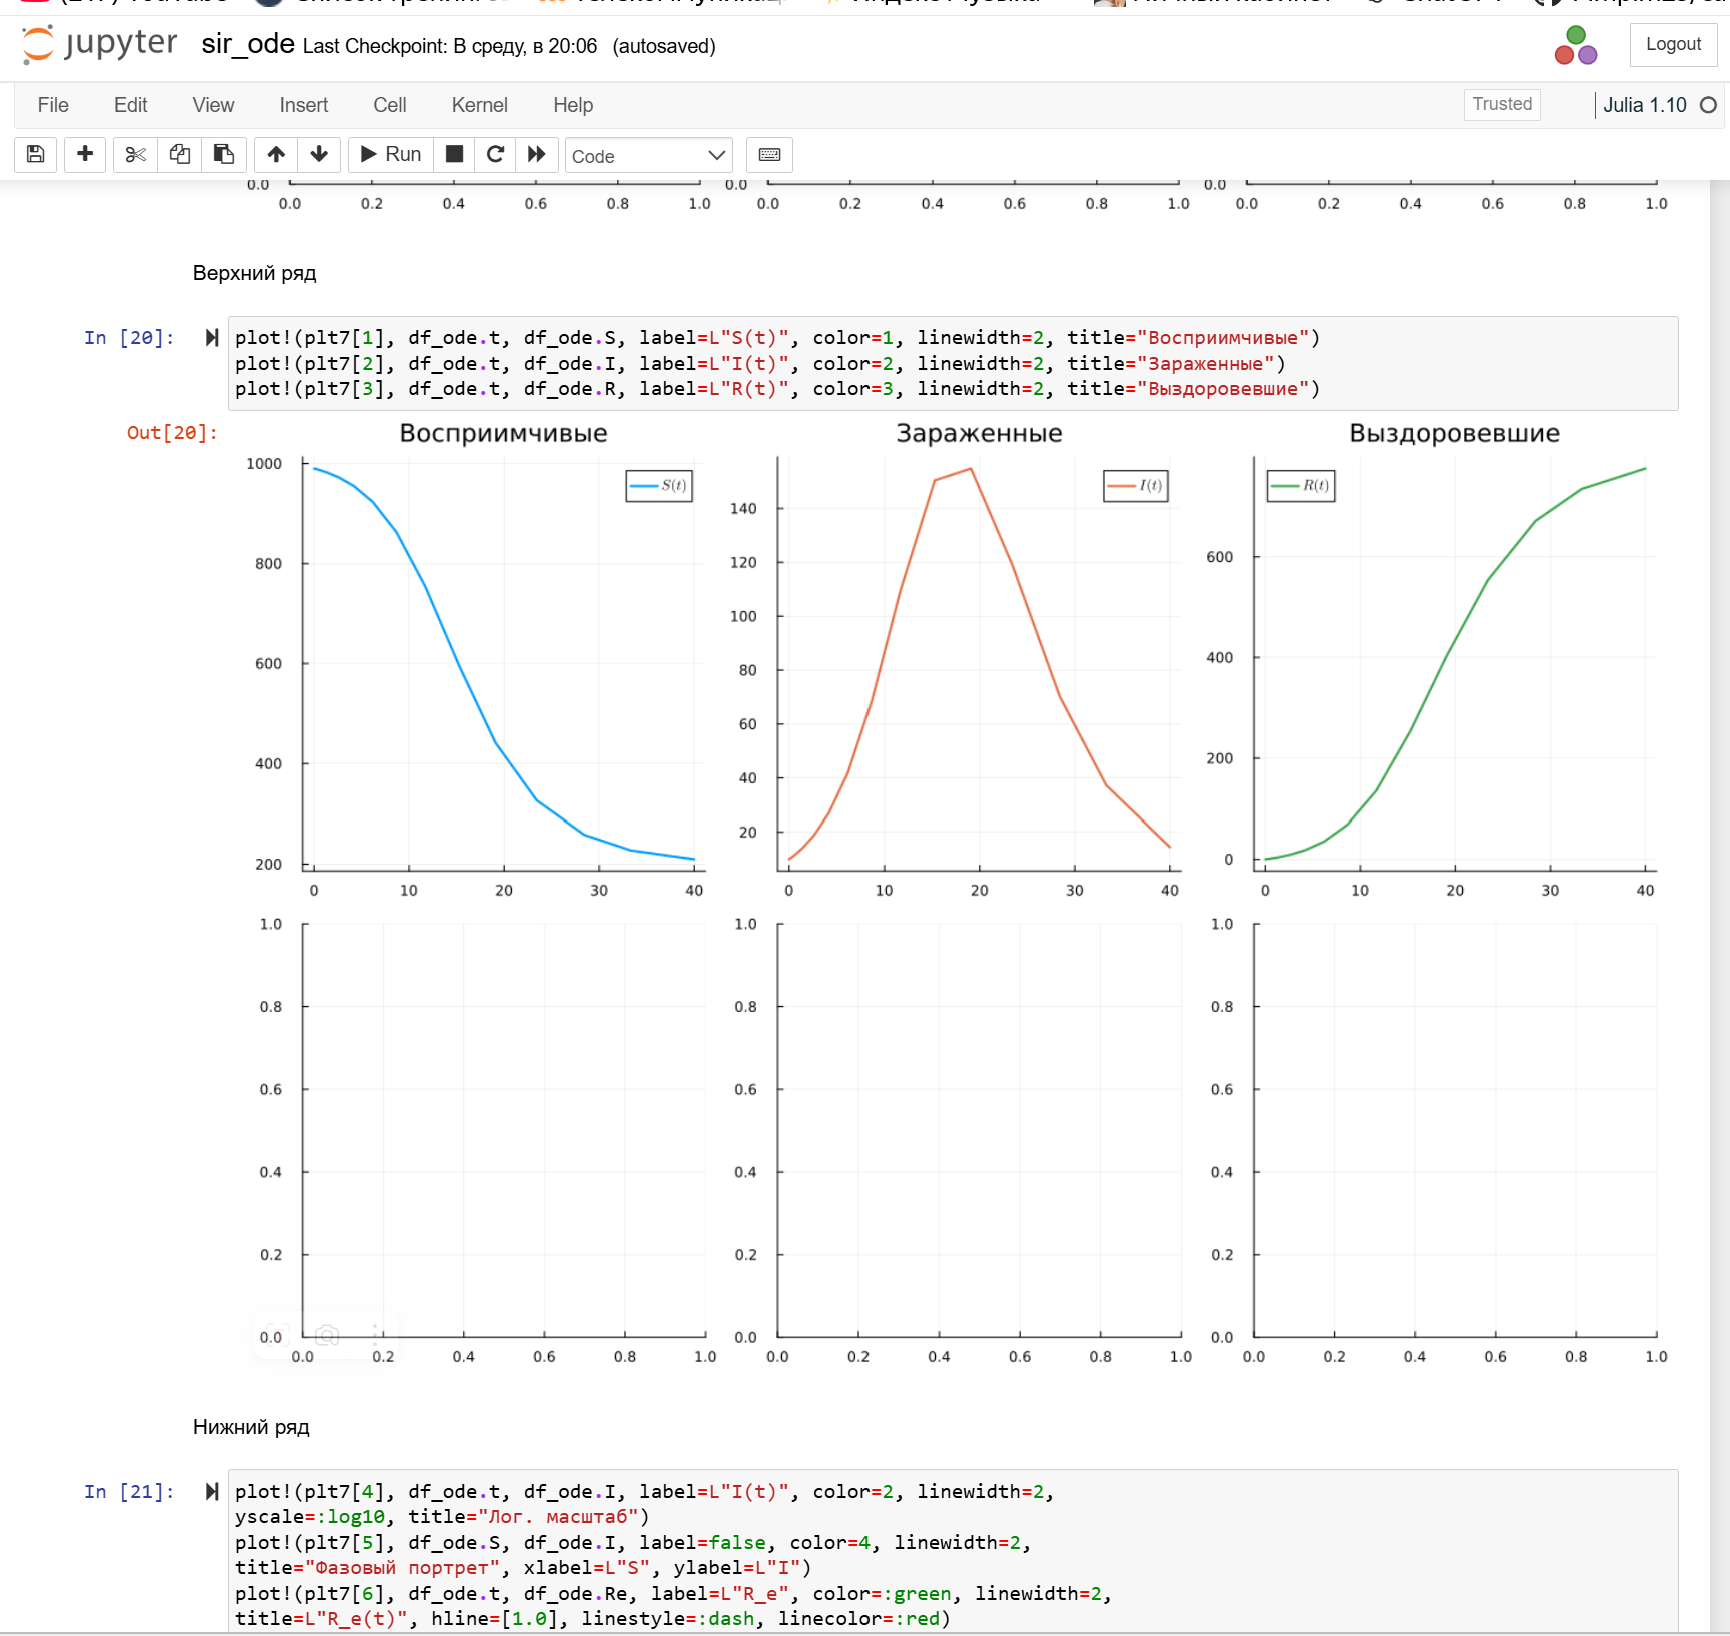
\includegraphics[width=0.7\linewidth,height=\textheight,keepaspectratio]{image/17.png}
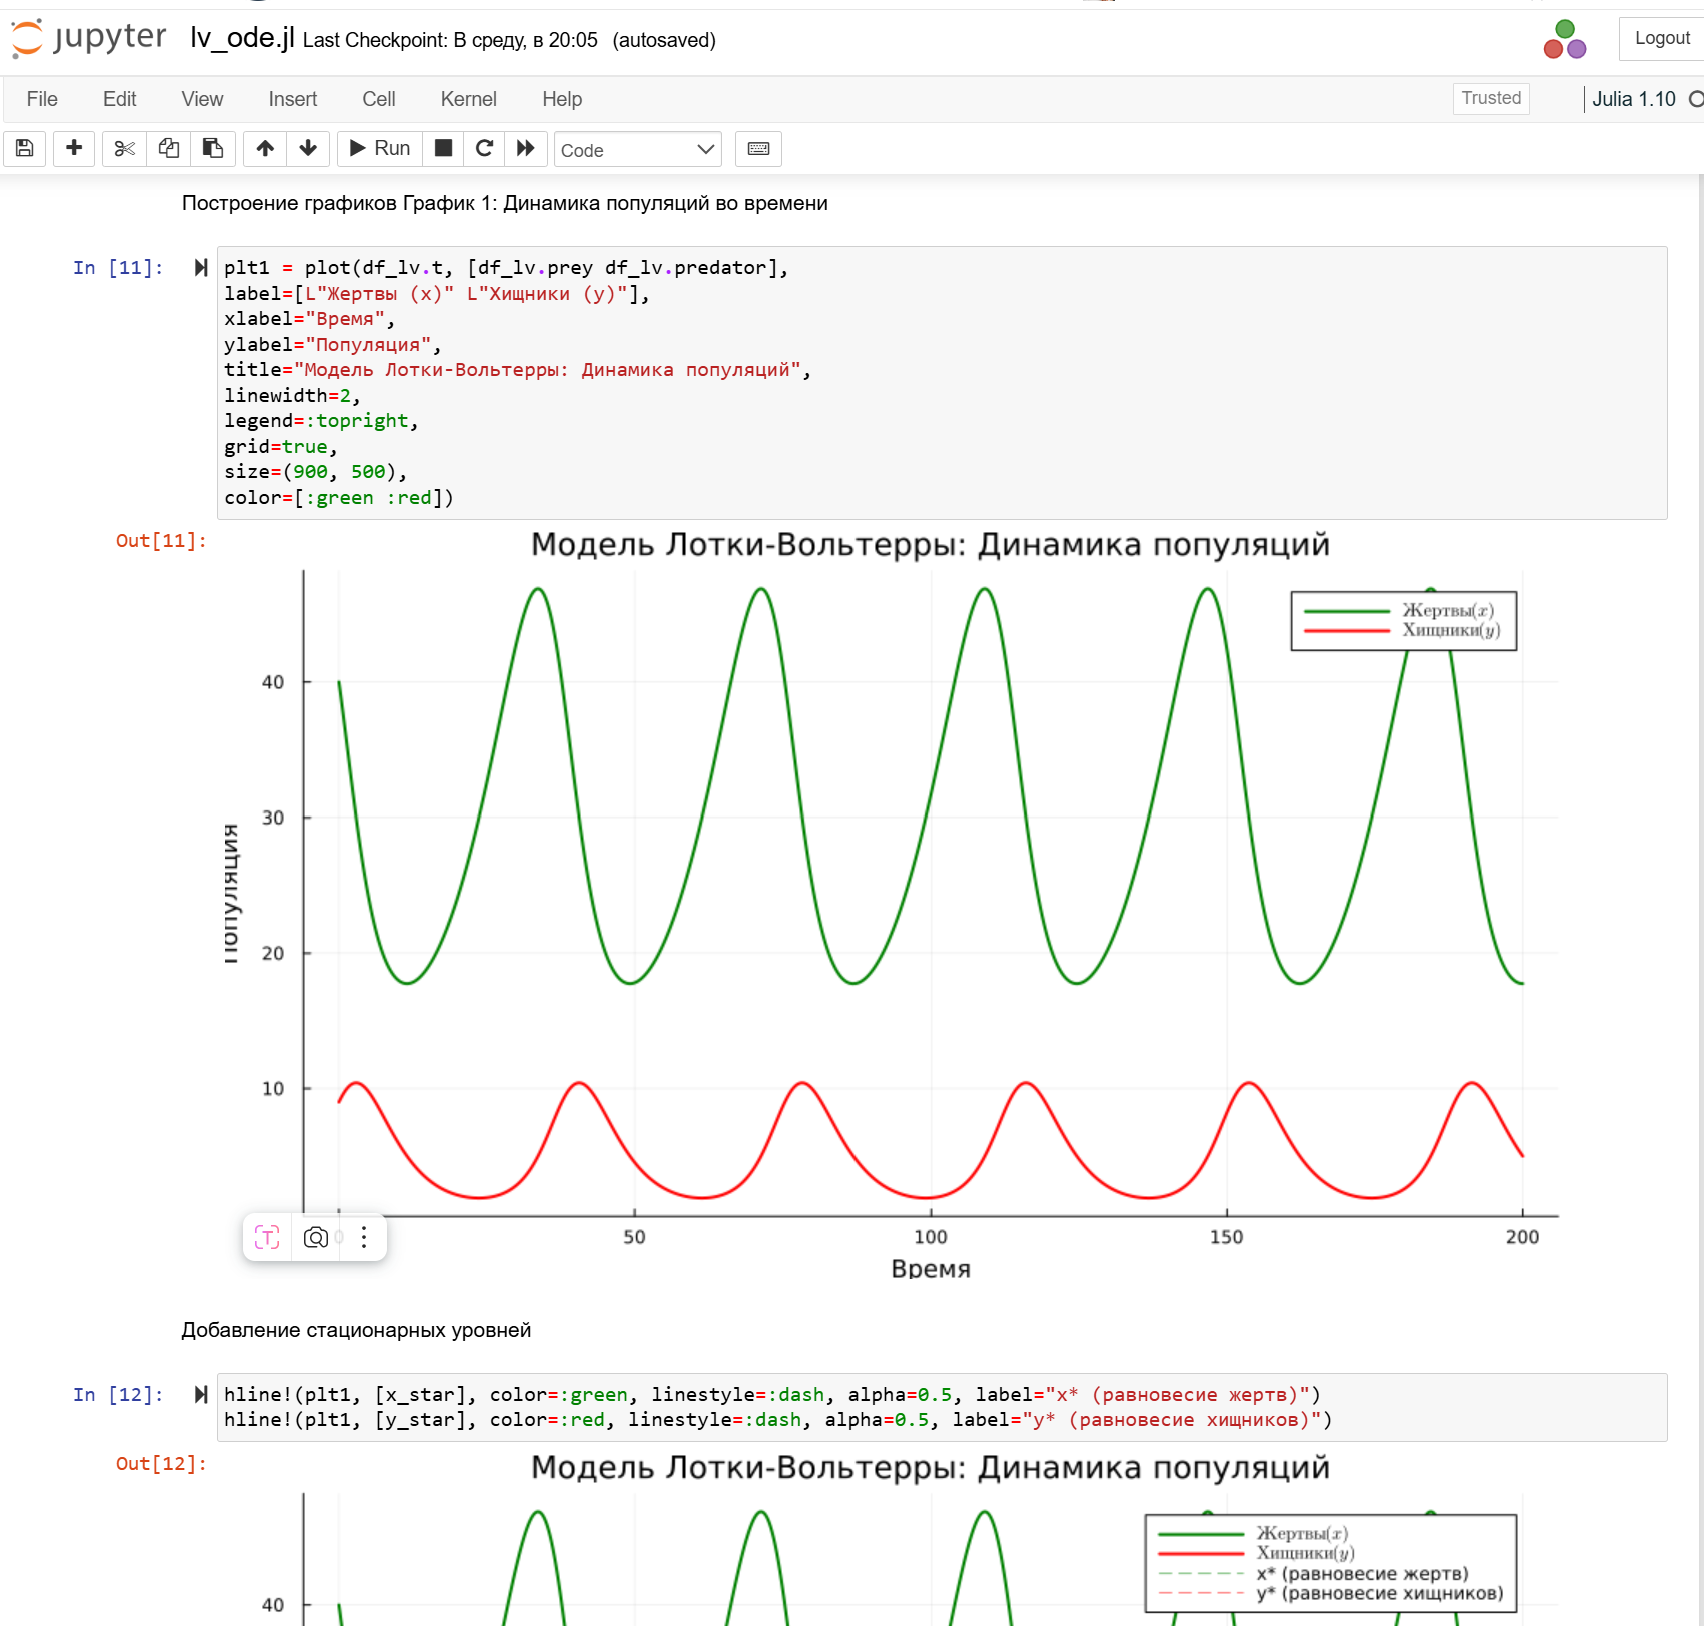
\includegraphics[width=0.7\linewidth,height=\textheight,keepaspectratio]{image/18.png}

\subsection{Настройка
Quarto}\label{ux43dux430ux441ux442ux440ux43eux439ux43aux430-quarto}

\begin{itemize}
\tightlist
\item
  Конфигурация \_quarto.yml
\end{itemize}

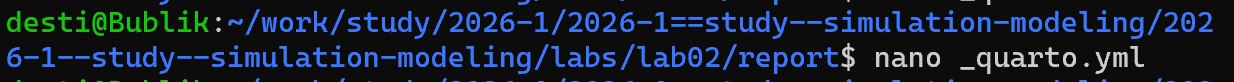
\includegraphics[width=0.7\linewidth,height=\textheight,keepaspectratio]{image/19.png}
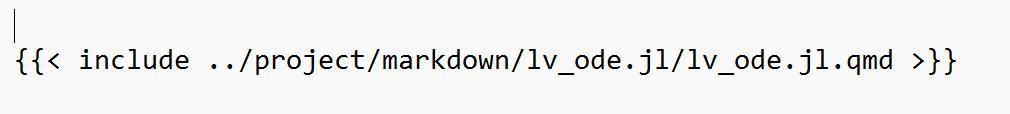
\includegraphics[width=0.7\linewidth,height=\textheight,keepaspectratio]{image/20.png}
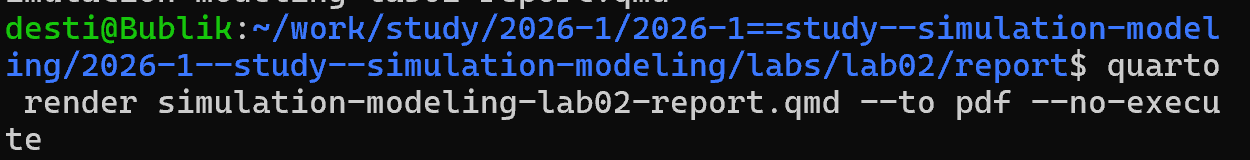
\includegraphics[width=0.7\linewidth,height=\textheight,keepaspectratio]{image/21.png}

\section{Результаты}\label{ux440ux435ux437ux443ux43bux44cux442ux430ux442ux44b}

\subsection{Модель SIR}\label{ux43cux43eux434ux435ux43bux44c-sir-2}

\begin{itemize}
\tightlist
\item
  Динамика эпидемии полностью определяется параметрами \(\beta\) и
  \(\gamma\)
\item
  Увеличение \(\beta\) или уменьшение \(\gamma\) повышает \(R_0\)
\item
  При \(R_0 > 1\) наблюдается эпидемический рост
\item
  При \(R_0 < 1\) вспышка затухает
\item
  Параметрическое исследование подтверждает теоретические зависимости
\end{itemize}

\subsection{Модель
Лотки-Вольтерры}\label{ux43cux43eux434ux435ux43bux44c-ux43bux43eux442ux43aux438-ux432ux43eux43bux44cux442ux435ux440ux440ux44b-2}

\begin{itemize}
\tightlist
\item
  Взаимодействие ``хищник-жертва'' носит циклический характер
\item
  Наблюдается сдвиг фаз между пиками жертв и хищников
\item
  Фазовый портрет --- замкнутая кривая (периодичность)
\item
  Изменение параметров влияет на амплитуду и период колебаний
\end{itemize}

\subsection{Методологические
результаты}\label{ux43cux435ux442ux43eux434ux43eux43bux43eux433ux438ux447ux435ux441ux43aux438ux435-ux440ux435ux437ux443ux43bux44cux442ux430ux442ux44b}

\begin{itemize}
\tightlist
\item
  Освоен фреймворк \textbf{DrWatson.jl} для организации проектов
\item
  Применено литературное программирование с \textbf{Literate.jl}
\item
  Созданы самодокументируемые скрипты
\item
  Сгенерированы Jupyter notebooks и Quarto-документы
\item
  Подтверждена эффективность Julia для решения ОДУ
\end{itemize}

\section{Рекомендации}\label{ux440ux435ux43aux43eux43cux435ux43dux434ux430ux446ux438ux438}

\subsection{Принципы организации
работы}\label{ux43fux440ux438ux43dux446ux438ux43fux44b-ux43eux440ux433ux430ux43dux438ux437ux430ux446ux438ux438-ux440ux430ux431ux43eux442ux44b}

\begin{itemize}
\tightlist
\item
  Использовать Git-flow для управления версиями
\item
  Применять Conventional Commits для автоматической генерации changelog
\item
  Регулярно запускать \texttt{tangle.jl} для обновления отчётов
\item
  Хранить только исходники в репозитории, генерируемые файлы --- в
  релизах
\end{itemize}

\subsection{Дальнейшие
исследования}\label{ux434ux430ux43bux44cux43dux435ux439ux448ux438ux435-ux438ux441ux441ux43bux435ux434ux43eux432ux430ux43dux438ux44f}

\begin{itemize}
\tightlist
\item
  Модификация SIR: SEIR, SIRS, модели с вакцинацией
\item
  Модификация Лотки-Вольтерры: внутривидовая конкуренция, ограниченные
  ресурсы
\item
  Стохастические версии моделей
\item
  Калибровка моделей по реальным данным
\end{itemize}

\section{Итоговый
слайд}\label{ux438ux442ux43eux433ux43eux432ux44bux439-ux441ux43bux430ux439ux434}

\subsection{Выводы}\label{ux432ux44bux432ux43eux434ux44b}

В результате выполнения лабораторной работы:

Изучены фундаментальные модели SIR и Лотки-Вольтерры\\
Реализовано численное решение на Julia\\
Проведён анализ влияния параметров на динамику систем\\
Освоены современные инструменты: DrWatson, Literate, Quarto\\
Подготовлен отчёт и презентация

\begin{center}\rule{0.5\linewidth}{0.5pt}\end{center}

Главное сообщение: \textbf{Julia и её экосистема предоставляют
эффективные средства для имитационного моделирования и воспроизводимых
научных исследований}




\end{document}
